\documentclass[11pt,a4paper,english]{report}

\usepackage{vpl}
\usepackage{mathpazo}
\renewcommand*\familydefault{\rmdefault}

\graphicspath{{../images/}}

% Inline block (graphics)
\newcommand*{\scrblk}[2][-5]{\raisebox{#1pt}%
{\includegraphics[scale=1]{#2}}}

% Scratch project name
\newcommand*{\scrprj}[1]{{\raggedleft\hfill Scratch project: \bu{#1}}}

%\includeonly{}

\begin{document}
% !TeX root = vpl.tex

\thispagestyle{empty}

\begin{center}
\begin{Huge}
\begin{bfseries}
Scratch Simulations

of the

Thymio Robot

\end{bfseries}
\end{Huge}

\vskip 2cm

\begin{LARGE}
\href{http://www.weizmann.ac.il/sci-tea/benari/}{Moti Ben-Ari}\\% and other contributors\\
\end{LARGE}
%\bigskip
%\begin{Large}
%see \texttt{authors.txt} for details
%\end{Large}

\vskip 1cm

\begin{Large}
Version 1.0 for\\
\bigskip
\href{https://aseba.wikidot.com/en:downloadinstall}{Aseba 1.4}\\
\bigskip
\href{https://scratch.mit.edu/}{Scratch 2.0}
\end{Large}

\end{center}

\vfill

\begin{center}
\copyright{}\  2015 by \href{http://www.weizmann.ac.il/sci-tea/benari/}{Moti Ben-Ari}.% and other contributors.
\end{center}

This work is licensed under the Creative Commons
Attribution-ShareAlike 3.0 Unported License. To view a copy
of this license, visit
\url{http://creativecommons.org/licenses/by-sa/3.0/}
or send a letter to Creative Commons, 444 Castro Street, Suite 900,
Mountain View, California, 94041, USA.

\begin{center}

\includegraphics[width=.2\textwidth]{by-sa}
\end{center}

\newpage
\begin{spacing}{0.7}
\tableofcontents
\end{spacing}
\thispagestyle{empty}
\newpage
\setcounter{page}{1}

\chapter*{Preface}
\addcontentsline{toc}{chapter}{Preface}

\sect{VPL and Scratch}

VPL is a visual programming environment for the Thymio robot
(Figure~\ref{fig.vpl}). Scratch (Figure~\ref{fig.scratch}) is a
web-based visual programming environment that animates \emph{sprites} on
the computer screen. The two environments have similar features: a
program is created by dragging-and-dropping blocks onto the screen, and
the fundamental programming construct is the \emph{event handler}.
Therefore, knowledge of one environment can be helpful in learning the
other.

\begin{figure}[hb]
\centering
    \subfigure[VPL]{
		\label{fig.vpl}
		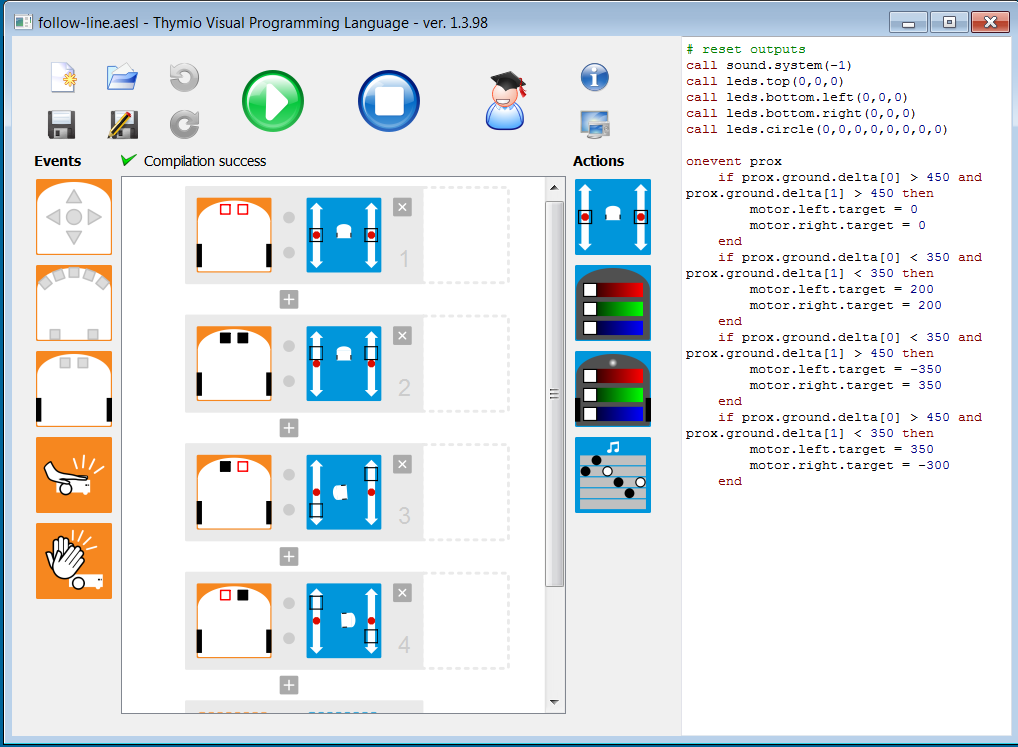
\includegraphics[width = 0.4\textwidth]{gui}
	}
	\hspace{1.5cm}
    \subfigure[Scratch]{
		\label{fig.scratch}
		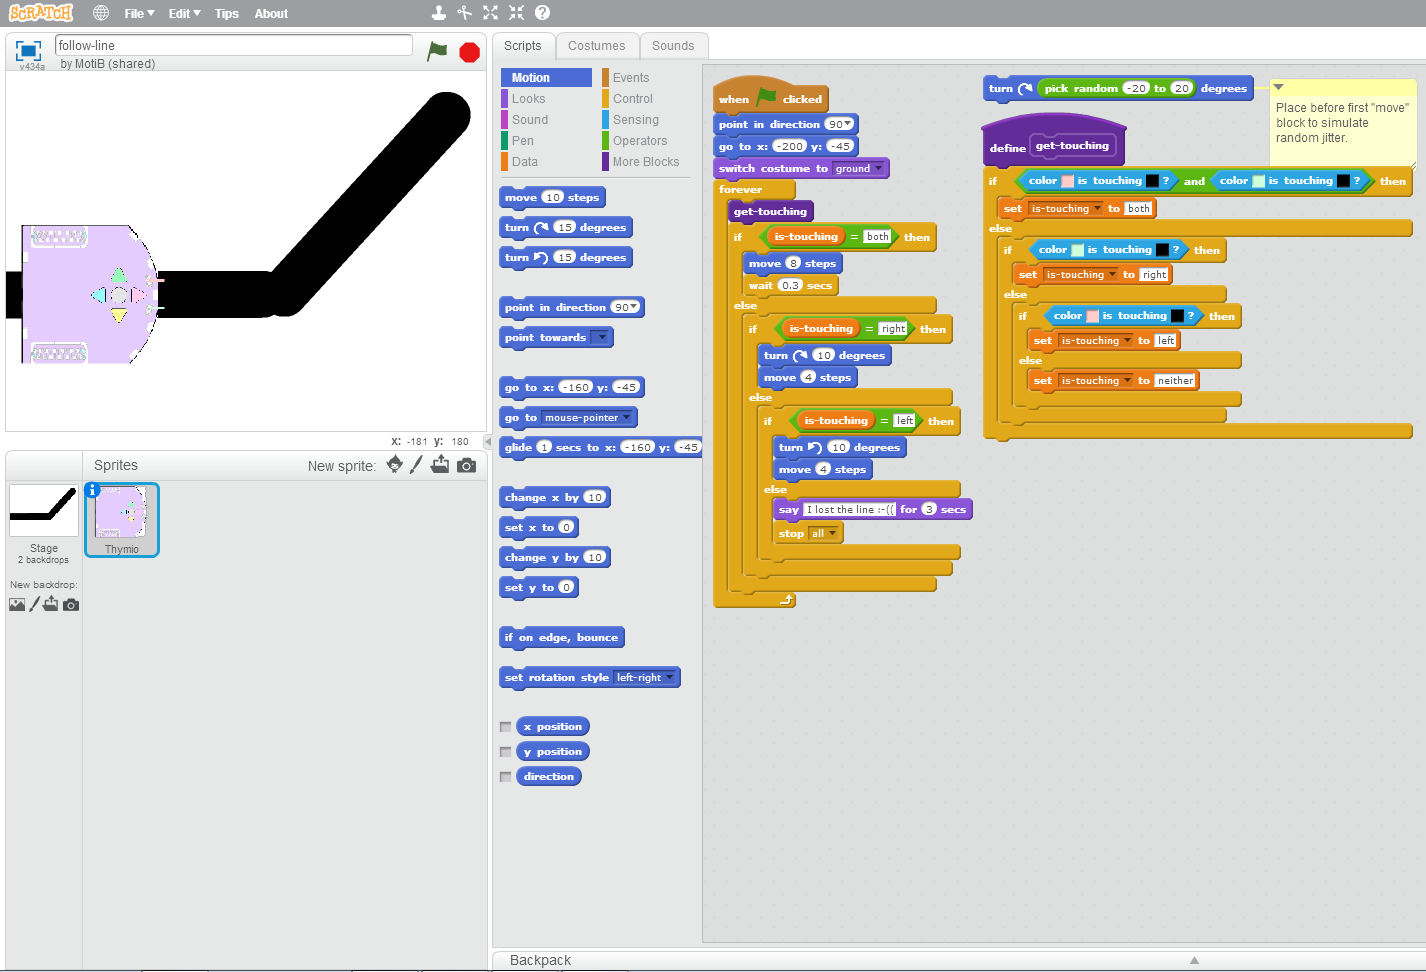
\includegraphics[width = 0.4\textwidth]{scratch}
	}
    \caption{VPL and Scratch}
    \label{fig.vplscratch}
\end{figure}

This document is about transfer from VPL to Scratch. It takes programs
from the VPL tutorial \emph{First Steps in Robotics with the Thymio-II
Robot and the Aseba/VPL Environment}
(\url{https://aseba.wikidot.com/en:thymioprogram}) and shows how to
implement them as Scratch programs controlling a sprite that is an
image of the Thymio robot.

\sect{References}

The document is not intended as a tutorial on Scratch, but
rather as a collection of projects that can be used when learning
Scratch. For an introduction to Scratch I recommend \textit{Computer
Science Concepts in Scratch} by Michal Armoni and Moti Ben-Ari, which
can be downloaded for free at
\url{http://stwww.weizmann.ac.il/g-cs/scratch/scratch_en.html}.

The projects are arranged in increasing complexity of the Scratch
implementation, not in the order they appear in the VPL tutorial.

The Scratch projects described here can be found on my website
(\url{http://www.weizmann.ac.il/sci-tea/benari/software/scratch/index.html}),
or in my Thymio studio on the Scratch website
(\url{http://scratch.mit.edu/studios/1023692}). For other
robotics-related Scratch projects, see my website or my Robotics
Studio (\url{http://scratch.mit.edu/studios/520857}).

\sect{On the implementation}

Aside from the obvious difference between the concrete Thymio robot and
its image on the Scratch stage, the main difference between the robotic
projects and the Scratch projects is how the sensors are implemented in
Scratch. Full details of the implementation are given in
\cref{ch.implementation}, but it is not necessary to understand them,
since a set of abstractions has been introduced and they will be
described as they are introduced in the projects.

\begin{itemize}

\item A sprite called \p{Pointer} is used to sense where the mouse is
clicked. It broadcasts the messages \p{center}, \p{front}, \p{back},
\p{left}, \p{right} to simulate touching the buttons.

\item The new block \scrblk[-6]{get-pointer-direction-block} returns in the
variable \scrblk[-4]{direction-to-pointer} the direction from the
\p{Thymio} sprite to the point where the mouse was clicked.

\item The new block \scrblk[-6]{get-touching-block} returns in the variable
\scrblk{is-touching} an indication if the \p{left} or \p{right} ground
sensors are touching a black tape, or if \p{both} sensors or \p{neither}
sensor are touching the tape.

\end{itemize}

The following costumes are used:

\begin{itemize}

\item The \p{Thymio} sprite is colored violet to make it stand out on the
stage. You can this color if you like. The buttons are colored and these
colors should not be changed.

\item Five costumes (\p{blank}, \p{red}, \p{green}, \p{blue},
\p{yellow}) simulate the top lights.

\item The costume \p{ground} simulates the ground sensors.

\end{itemize}

\chap{Programming with Events}\label{ch.events}

\sect{Events}

\scrprj{tap-on-off}

In VPL an instruction consists of an event block followed by one or
more action blocks:

\gr{first}{.3}

\emph{Each time} the event occurs, the actions associated with the event
are performed. Here, when the front button of the robot is touched, the
top light is turned on with color red, and when the back button is
touched, the light becomes blue.

In Scratch, the construction equivalent to an event-actions pair is the
\emph{script}:

\gr{tap-on-off}{.3}

The image shows three scripts, each of which changes the costume of the
sprite:

\begin{itemize}

\item Scratch programs are started by clicking on the \emph{green flag}
above the stage. When the green flag is clicked, the costume of the
sprite is set to the \p{blank} costume, which displays the Thymio with
the top lights off.

\item The second script responds to the event of pressing the \bu{r}
key. The costume is changed to the \p{red} costume which displays the
top lights in red.

\item Similarly, the third script turns the lights blue when the \bu{b}
key is pressed.

\end{itemize}

The \bu{Events} palette contains the event blocks which are colored
brown. Most of these blocks have a ``hat'' shape to indicate that they
can only be the first block in a script. After an initial event block,
other blocks can be added to the script.


\sect{Costumes}

A sprite can have one or more \emph{costumes} which specify how the
sprite is displayed on the stage. The sprite's costumes are displayed
when you click the \bu{Costumes} tab. You can create costumes by
importing images, or by drawing or editing them using a paint program
that is included in Scratch.

\informationbox{The costumes for this project}{The project
\bu{thymio-costumes} contains all the costumes used in these projects.
Open this project and copy (drag and drop) the costumes you need to your
\bu{Backpack}. Now open a new project and copy the costumes to the
sprites.}

\informationbox{Setting the size of the costumes}{You may have to adjust
the size of the image of the sprites in order for a project to work. You
can do this by shrinking a costume in the paint program: click on the
icon \scrblk{shrink} and then on the image. A better solution is to use
the block \scrblk[-10]{set-size} from the \bu{Looks} palette in the initialization
of a program; experiment with different values until you have the size the need.}

\sect{Sending and receiving messages}

\scrprj{colors}

Let us look now at the program \bu{colors} which changes the color of
the top lights according to which button is touched
(Figure~\ref{fig.colors}). In Scratch, touching a button is simulated by
clicking on the image of a button. The click is interpreted by a second
sprite called \p{Pointer}, which sends a message to the \p{Thymio} sprite,
depending on which image is clicked: \p{center}, \p{front}, \p{back},
\p{left}, \p{right}.

\begin{figure}
\gr{colors}{.25}
\caption{Changing colors using messages}\label{fig.colors}
\end{figure}

Click on the \p{Pointer} sprite in the sprite area in the lower left of
the Scratch window. Without going into detail, just notice that the
second script uses the block \scrblk[-8]{broadcast-and-wait}, which causes
a message (here, \p{front}) to be sent. Now, click back on the \p{Thymio}
sprite and you will see the scripts in Figure~\ref{fig.colors}. Scripts
starting with the event block \scrblk{when-i-receive} are performed when
the corresponding message is received. We see that different messages
cause the costume of the \p{Thymio} to be changed to ones displaying
different colors.

\sect{Sounds}

\scrprj{bells}

The VPL project \bu{bells} caused notes to be played when the buttons
are touched. In Scratch, the \bu{Sound} palette contains a rich set of
blocks for playing notes. Experiment with these blocks and then replace
the blocks that change costumes in the above project with blocks that
play different sounds when different buttons are clicked. You can also
add sound blocks to the script in Figure~\ref{fig.colors}, so that the
sprite both changes colors and plays sounds.

\chap{Moving Sprites}\label{ch.moving}

\scrprj{moving}

In the project \bu{moving}, the robot moves forwards and backwards when
the front and back buttons are touched, and it stops when the center
button is touched. In Scratch, a sprite will move on the screen in
response to running blocks from the \bu{Motion} palette.

The following script initializes the sprite to start at the left
side of the stage, pointing right ($90^{\circ}$):

\gr{moving1}{.3}

The size of the stage is from $-240$ to $240$ pixels (picture elements)
in the $x$ (horizontal) direction and $-180$ to $180$ pixels in the $y$
(vertical) direction. You can explore these values by moving your mouse
around the stage; its position is displayed below the lower right corner
of the stage. The initial position of the \p{Thymio} sprite is set to
$(-100,0)$, so that it is at the left edge of the stage and centered
vertically.

The sprite runs the following script when it receives the message
\p{front} that is broadcast when the front button is clicked:

\gr{moving2}{.3}

The block \scrblk{move} is contained within a
\scrblk[-10]{forever} block that causes the instruction to be run
repeatedly. This will cause the sprite to move steadily in the direction
it is pointing.

The \scrblk{wait03} block causes the program to wait 0.3 seconds before
continuing with the next block. This slows down the movement and makes
it easier to click on a button.

The script for responding to the \p{back} message is the same as that
for the front message, except that the sprite is made to point left
($-90^{\circ}$):

\gr{moving3}{.3}

When the \p{center} message is received, all the scripts in the
program are stopped:

\gr{moving4}{.3}

\warningbox{Turning the sprite to move in the direction $-90^{\circ}$
will also cause the \emph{image} of the sprite to turn $180^{\circ}$. To
prevent this, select the \p{Thymio} sprite icon in the area below the
stage and click on the small \bu{i} in the icon. Then click on the dot
which is one of the options in \bu{rotation style}.}

\sect{Directions}

\scrprj{obeys}

The \p{Thymio} can behave like a pet, following you around. In project
\bu{obeys}, click the mouse closer and closer to the center sensor on
the image of the \p{Thymio} sprite. When it is close enough, the red light
on the sensor turns on and the robot moves towards the pointer, stopping
when it is close.

Initialize the project as in \bu{moving} adding the block
\scrblk{switch-costume-to-blank}. The main script for this project is
shown in \cref{fig.move-to}. The script starts running when it receives
the message \p{Come}, which is sent by the \p{Pointer} sprite when the mouse
is clicked.

\begin{figure}
\gr{obeys}{.75}
\caption{Move towards an object near the center sensor}\label{fig.move-to}
\end{figure}

\subsection*{Distance to a sprite}

The robot moves only when it detects that the pointer is close. The
sprite \p{Pointer} tracks the mouse pointer. The block
\scrblk[-4]{distance-to-pointer} returns the distance in pixels from the
sprite that runs it---here the \p{Thymio} sprite---to the \p{Pointer} sprite.
The block can be found in the \bu{Sensing} palette.

Next, we compare this distance with the distance $250$ that we decide is
``close'' enough to be detected. In the palette \bu{Operators} you can
find mathematical operators for performing comparisons:
\scrblk{distance-less-than}.

The block with comparison operator is a \emph{condition block}. The
\p{if} block \scrblk[-15]{if} has an angular area for a condition block
and a ``mouth'' in which you can place other blocks. The meaning of the
\p{if}-block is:

\begin{footnotesize}
\begin{verbatim}
if the condition is true then
    the blocks contained in the "mouth" are run.
\end{verbatim}
\end{footnotesize}

It follows that the rest of the blocks in the script in
\cref{fig.move-to} will be run only when the \p{Pointer} sprite is close to
the \p{Thymio} sprite.

\subsection*{Direction to a sprite}

The specification requires that the Thymio respond only if the pointer
is detected in front of the center sensor. This is implemented by
calling the block \scrblk[-6]{get-pointer-direction-block} which returns in
\scrblk[-4]{direction-to-pointer} the direction of the \p{Pointer} from the
front of the \p{Thymio} sprite. Its value is in degrees in the range 0 to
360, clockwise; that is, directions just to the right of the \p{Thymio} will
have low values, while directions just to the left of the \p{Thymio} will
have values close to $360$. We decide that the \p{Pointer} is detected by
the center sensor if the direction is greater than $325$ or less than $25$.

\informationbox{User-defined
blocks}{\scrblk[-6]{get-pointer-direction-block} and
\scrblk[-4]{direction-to-pointer} are not predefined in Scratch. The
implementation of these blocks is described in \cref{ch.implementation},
but you can use the blocks without understanding the implementation.}

A second \p{if}-block is used to run blocks only when the direction to
the \p{Pointer} is greater than $325$ or less than $25$. The \bu{Operators}
palette contains the operator \scrblk{or} which enables us to combine
the two conditions into one. The result is a \emph{compound condition}
that is true if either of its parts is true.

If the compound condition is true, we turn the \p{Thymio} to face the
\p{Pointer} sprite using the block \scrblk[-6]{point-towards-pointer} from the
\bu{Motions} palette, and we change the costume so that the red light
next to the center sensor is turned on.


\subsection*{Approaching a sprite}

If the \p{Thymio} sprite is close to the \p{Pointer} sprite and is pointed in
the right direction, the robot must approach the sprite. We use
\scrblk[-15]{repeat-until} which is similar to the \p{forever} block in
that it causes the blocks contained in its ``mouth'' to be run again and
again, but it is different in that it has a condition like an
\p{if}-block. The movement of the \p{Thymio} sprite must stop if the
distance to the \p{Pointer} sprite is too small and this is checked by
the condition block \scrblk[-8]{distance-to-pointer-60}.

\chap{Defining New Blocks}\label{ch.new}

\scrprj{likes}

The project \bu{likes} is similar to \bu{obeys} except that the
\p{Thymio} sprite turns towards the object when one is detected by the
left or right sensors and not just by the center sensor:

\begin{footnotesize}
\begin{verbatim}
if center sensor faces Pointer
    switch costume to center
    go to Pointer
else
  if right sensor faces Pointer
      switch costume to right
      go to Pointer
  else
    if left sensor faces Pointer
      switch costume to left
      go to Pointer
\end{verbatim}
\end{footnotesize}

In Scratch, we can define new blocks such as
\scrblk[-8]{go-to-pointer-block}. Once the block is defined, we can use it
to write the script for \bu{likes} (\cref{fig.likes}).

\begin{figure}
\gr{likes}{.75}
\caption{Script for \bu{likes}}\label{fig.likes}
\end{figure}

How do we define the new block? Go to the palette \bu{More Blocks} and
click on \scrblk{make-block}. Enter the name of the new
block, \p{go-to-pointer}, in the purple field in the \p{New block} window
that is opened. This will create the block \scrblk[-10]{define-go-to-pointer}
block in the script area and the \scrblk[-8]{go-to-pointer-block} in the block
area for this palette. Now you can drag-and-drop the blocks required to
implement the new block (\cref{fig.go-to}).

\trickbox{When defining a new block, click on \bu{Options} and \bu{Run
without screen refresh}. This ensures that the new block is run as one
action and the user does not see the result of running each block in the
definition.}

The new block \scrblk[-8]{go-to-pointer-block} can be used in different
scripts and even more than once in the same script as shown in
\cref{fig.likes}. Clearly, this script is much shorter than it would be
if we had to copy the blocks again and again.

\begin{figure}
\gr{go-to-pointer}{.5}
\caption{Definition of the block \bu{go-to-pointer}}\label{fig.go-to}
\end{figure}

\chap{Variables}\label{ch.variables}

\sect{Using a variable to store a state}

In advanced mode, VPL projects can use \emph{states} to remember
situations and values. There are four elements (``quarters'') to the
state block, so there are 16 different states. Scratch supports
\emph{variables} which can be used to store values. They offer many more
capabilities than VPL states, because there can be as many variables are
use want and each variable can store a large range of values.

\scrprj{tap-on-off-state}

Let us implement the project \bu{tap-on-off} from the tutorial. Clicking
on the \p{Thymio} sprite will turn the top light on if it is off and turn it
off if it is on. A variable will remember the current state \p{on}
or \p{off}. First, we \emph{declare} the variable. Go to the \bu{Data}
palette and click \scrblk{make-variable}; give the variable a name that
makes clear what its purpose is. An oval block with
the variable's name appears, together with some new blocks:

\gr{declare}{.3}

\informationbox{Displaying the value of the variable}{The check box next
to the variable block is used to indicate if you want the variable and
its current value to be displayed on the stage or not.}

We need to \emph{initialize} the variable in the script that is
run when the green flag is clicked. This gives the variable a
value before it is used for the first time. Here, the block
\scrblk[-8]{set-block} sets the value to \p{off}:

\gr{tap-on-off-state-init}{.35}

The following script starts with the block \scrblk[-8]{when-sprite-clicked},
meaning that it begins to run when the sprite that contains the script is clicked:
 
\gr{tap-on-off-state}{.4}

It checks the value of the variable \p{state} and decides whether to
switch the costume to the red costume or to the blank costume. It also
changes the current value of the variable \p{state} to the opposite
value.


\sect{Using a variable to store a number}

\scrprj{count-to-two}

\scrprj{count-to-four-binary}

\scrprj{add}

Variables are commonly used to store numbers. The VPL project
\bu{count-to-two} encoded the numbers 0 and 1 in states, and later
projects counted to 4 and even to 16. We show how to use variables to
count to two in binary, and leave the extension to other numbers as
exercises.

The Thymio robot displays the current state by lighting the
diagonal segments of the circular lights around the buttons. We simulate
this by displaying an orange circle between the buttons on an image:

\gr{buttons-with-light}{.3}

There are two aspects to the simulation in Scratch: (1) initializing,
incrementing and checking the variable, and (2) displaying and erasing
the orange circle.

We first discuss the operations on the variable. The variable is named
\p{count} and is initialized to zero in the first script:

\gr{count-2-init}{.2}

In the second script, the choice whether to display or erase the circle
is done in an \p{if}-statement that checks if the value of
\scrblk{count-block} is 0 or not, using the \scrblk[-20]{if-else} block:

\gr{count-2}{.35}

If the condition is true, the blocks in the first ``mouth'' are run; if
not, the blocks in the second ``mouth'' are run.

The actual display of the circle is done within the two blocks
\scrblk{display-block} and \scrblk{erase-block} whose definition is
given below.

The final block of the script is \scrblk{change} which changes the
(numerical) value in the variable by the amount written in the small
square. Here, \scrblk{mod} adds 1 to the value of \scrblk{count-block}
and then takes the remainder (called \p{mod}) by 2. The result will be
either 0 or 1.

\warningbox{Be sure not to confuse \scrblk{set-one} with
\scrblk{change}. The first block ignores the current value in the
variable and sets the variable to the value written in the small square.
The second block takes the current value of the variable, adds the
value written in the small square and then sets the value of the
variable to the result of the computation. To subtract a value
from the current value, simply change by a negative number.}

\sect{Drawing on the stage}

Scratch supports drawing on the stage using blocks available in the
\bu{Pen} palette. We will not explain all the blocks here, just the ones
used to display and erase the orange circle.

In the initialization script, \scrblk{clear} erases existing marks on
the stage , if any. The blocks \scrblk{display-block} and
\scrblk{erase-block} contain \scrblk{stamp} which prints the image of
the current costume of the sprite on the stage:

\gr{display-erase}{.5}

\warningbox{Be sure not to confuse sprites and stamps.
A sprite is an actor in a Scratch animation; it has scripts and
costumes. When it moves on the stage it does not leave a mark.
The block \scrblk{stamp} makes a mark on the stage; the mark is the
current costume of the sprite that runs the block. The stamp is not an
actor and does not move, and the mark remains indefinitely on the stage
until removed by running \scrblk{clear}.}

Don't use the \scrblk{clear} when you only need to erase one mark such
as an orange circle. Instead, change the costume of the sprite to one
that is all white and stamp it in exactly the same place as the mark of
the orange circle.

The block \scrblk{hide} is used in the initial script because we don't
want to display the sprite, only the marks that it makes on the stage.

\sect{Why two sprites?}

There are two sprites in this project: a \p{Thymio} sprite (well, only
the buttons), and a \p{circle} sprite. The \p{Thymio}
sprite is the one that is clicked on; it broadcasts a message to the
\p{circle} sprite. We don't want to sense a click on the \p{circle}
sprite, because it may not be visible, and we don't want to stamp the
\p{Thymio} sprite because we want marks of the circle, not of the
buttons.

\sect{Parameters}

We want to use the blocks \scrblk{display-block} and
\scrblk{erase-block} in more than one place with different values for
the positions of the marks. The definitions of the blocks
\scrblk[-15]{display-head} and \scrblk[-20]{erase-head} declare two
\emph{parameters} called \p{x} and \p{y}. When the blocks are used, the
x- and y-values of the position need to be provided in the small
squares, just as is done in predefined blocks like \scrblk{go-to-block}.

Within the definition of a block with parameters, the current values of
the parameters are available as oval blocks that can be used like any
other variable.

\chap{Guided Projects}\label{ch.projects}

These projects introduce no new concepts so we present them as a guided
projects.

\sect{Line following}

\scrprj{follow-line}

Construct a backdrop with a wide line that represesnts a strip of black
tape on the floor:

\gr{line}{.2}

Next, import the costume called \p{ground}:

\gr{ground}{.2}

This costume has two small areas projecting from the front of the robot
and is used to implement the block \scrblk[-6]{get-touching-block} as
described in \cref{ch.implementation}. The block returns in the variable
\scrblk{is-touching} one of \p{both}, \p{left}, \p{right}, \p{neither}
depending on which projecting area is touching the black area on the
stage. The \p{Thymio} sprite needs one script whose algorithm is shown
in \cref{fig.line-following}.

\begin{figure}
\begin{footnotesize}
\begin{verbatim}
initialize the position of the Thymio
forever
    call get-touching-block
    if is-touching = both
        move forward
    else
        if is-touching = right
            turn right
        else
            if is-touching = left
                turn left
            else
                stop the script
\end{verbatim}
\end{footnotesize}
\caption{Algorithm for line following}\label{fig.line-following}
\end{figure}

\subsection*{Real robots don't move straight}

From your experience with the Thymio robot, you know that it will not
move straight even if both motors are set to the same power. The wheels
and motors are not identical, the friction may vary, and so on. This
noisy behavior is called \emph{jitter}. Place the following block before
first \p{move} block to simulate random jitter:

\gr{jitter}{.4}

The block causes the robot to turn by an angle that is randomly chosen
in the range $-20$ to $20$. You will see that the robot moves very
erratically, but the algorithm succeeds in keeping the robot on the line.


\sect{Sweeping the floor}

\scrprj{sweep}

We want the \p{Thymio} sprite to traverse the stage so as to cover the
whole surface:

\gr{sweep-stage}{.3}

In order the evaluate the quality of the sweep, the robot draws a thin
red line as it moves. \scrblk{pen-down} causes an imaginary pen in the
sprite to be lowered ``down'' so that it is in contact with the stage.
We also choose to set the pen color to red.

The simulation could be programmed simply by commanding the
sprite to move the correct distances---$280$ steps horizontally and
$60$ steps vertically---turning right and left by $90^{\circ}$ as
required. However, there is no way to command the Thymio \emph{robot} to
travel a certain distance. All we can do is to set the motors to a
constant power for a fixed time, but the speed will not be precisely
constant for the reasons mentioned above, so the distance will not be
predictable.

\begin{figure}
\gr{sweep1}{.35}
\caption{Sweeping the stage}\label{fig.sweep}
\end{figure}

The script shown in \cref{fig.sweep} causes the sprite to move 4 steps
at a time. A second script (not shown) consists of a
\scrblk[-15]{repeat-until} block that contains blocks for left and right
turns of $90^{\circ}$ with \scrblk{wait03} blocks between them. Adjust
the durations in the \p{wait} blocks to obtain a good sweep of the
stage.

\sect{Finite automata}

\scrprj{finite-automaton}

The finite automata project in the VPL tutorial was inspired by the
light-painting projects described on the Thymio website. The idea is to
have the robot sweep over an area and respond to codes placed on the
floor. The code consists of synchronization marks and marks of symbols
on the stage. \cref{fig.fa} shows the stage with 4 rows of 4 sync marks
(the blue circles) and 9 vertical black lines representing the symbol 1.

\begin{figure}[htb]
\gr{fa-stage}{.3}
\caption{Synchronization and symbol marks}\label{fig.fa}
\end{figure}

\newpage

The \p{Thymio} sprite is required to sweep the stage and record the number
of 1's. (For a finite automata we need to specify a finite range, such
whether the number of 1 symbols is even or odd. This can be done using
the \p{mod} operator.)

The sprite can be in three states: (1) it is touching a sync mark alone,
(2) it is touching both a sync mark and the black line encoding 1, and
(3) it is touching neither. Use \scrblk{touching-color-blue} to detect
the blue ball representing the sync marks and
\scrblk{touching-color-black} to detect black line representing 1.

To check the behavior of the sprite,
display different colored top lights in each state.

\warningbox{The sync marks should be sufficiently far apart so that
the \p{Thymio} sprite doesn't touch two two marks at the same time.}

\subsection*{Synchronizing the sprites}

There will be two sprites: the \p{Thymio} sprite that sweeps the floor
and decodes the marks, and a \p{ball} sprite that stamps marks on the
stage before the \p{Thymio} sprite starts to move. Use messages to
synchronize the sprites:

\begin{itemize}
\item The \p{Thymio} sprite performs initialization and then
broadcasts the message \p{draw}.
\item When the \p{ball} sprite receives the \p{draw} message, it stamps the
marks and then broadcasts the message \p{go}.
\item When the other scripts in the \p{Thymio} sprite receive the
\p{do} message, they begin the tasks of sweeping the stage and decoding
the marks.
\end{itemize}

\sect{Timed behavior}

\scrprj{shy}

Specification: If the \p{Pointer} is clicked opposite the right sensor,
the \p{Thymio} sprite turns until the \p{Pointer} is opposite the center
sensor and then 4 seconds later turns back. Similarly, if the
\p{Pointer} is clicked opposite the left sensor. Be sure that the small
red lights on the left, right and center sensors are turned on and off as
appropriate.

Guidance: The behavior for detection by the left and right sensors is
the same except for the costumes. Create a new block
\p{turn-and-turn-back} with one parameter---the direction---that
includes all the blocks needed to implement the behavior of the
\p{Thymio} sprite once the \p{Pointer} sprite is detected.

\newpage

\sect{Catch the mouse}

\scrprj{mouse}

Specification:

\begin{itemize}
\item The \p{Thymio} sprite detects a click of the \p{Pointer} sprite
opposite its left sensor.
\item It turns left (counterclockwise) until the right sensor points
towards the \p{Pointer}.
\item It turns right (clockwise) until the center sensor points towards
the \p{Pointer}.
\item It moves towards the point of the click and then stops.
\end{itemize}

Guidance:

\begin{itemize}

\item Declare a variable that will take four values:
\p{search-left}, \p{search-right}, \p{found}, \p{stop}. This variable
will take on successive values as it accomplishes each part of the
mission.

\item The behavior of the \p{Thymio} sprite will depend on which state
it is in. It is convenient to define new blocks for each state:
\p{go-left}, \p{go-right}, \p{catch-mouse}.

\end{itemize}

\appendix
\chap{Implementation}\label{ch.implementation}

This Appendix explains advanced programming techniques in Scratch that
were used in the simulations of the Thymio robot. The details are
encapsulated in sprites and new blocks so that the student need not be
concerned with them, but the Appendix can serve are a tutorial to these
programming techniques.

\sect{The {\ttfamily Pointer} sprite}

The \emph{touching} blocks from the \bu{Sensing} palette are used to
detect events. They are condition blocks that return true if the
\textbf{\emph{sprite running the script where the block appears}}
touches something else.

\begin{itemize}
\item \scrblk{touching} returns true if the sprite is touching another
sprite or the mouse pointer.

\item \scrblk{touching-color} returns true if the sprite is touching an area
with this color.

\item \scrblk{color-touching-color} returns true if an area
\textbf{\emph{on this sprite}} with the first color is touching an area
with the second color.

\end{itemize}

\trickbox{To set the color, click the little square,
move the mouse pointer and click an area on a sprite or the
backdrop that has the color you want.}

Scratch does not support checking if the mouse pointer is touching
a color; therefore, we define a sprite called \p{Pointer} that tracks
the location of the mouse pointer (\cref{fig.track}). The costume of
this sprite is a very small gray dot that the user will not see.

\begin{figure}[htb]
\gr{go-to-mouse-pointer}{.25}
\caption{Tracking the mouse pointer}\label{fig.track}
\end{figure}

To simulate the buttons on the Thymio robot, the image of the \p{Thymio}
sprite has different colors for each button. When the \p{Pointer} sprite
is clicked, the script in \cref{fig.buttons} checks if it is touching
one of the colors and broadcasts the appropriate message.

\begin{figure}[htb]
\gr{click-on-buttons}{.3}
\caption{Sensing a click on the buttons}\label{fig.buttons}
\end{figure}


\sect{Computing the direction to the {\ttfamily Pointer} sprite}

Many projects require that the direction from the \p{Thymio} sprite to
the \p{Pointer} sprite be determined. The implementation of the block
\scrblk[-6]{get-pointer-direction-block} is shown in \cref{fig.get-dir}.
The variable \scrblk[-3]{save-dir} is used internally
by this block, and the variable \scrblk[-3]{direction-to-pointer} is
used to return the direction to the calling sprite. Extensive use is
made of the block \scrblk[-3]{direction} which is predefined in the
\bu{Motion} palette and gives the current direction in which the sprite
is pointing.

\begin{figure}[htb]
\gr{get-pointer-direction}{.5}
\caption{Get the direction to the \p{Pointer} sprite}\label{fig.get-dir}
\end{figure}

The \emph{current direction} in which the sprite is pointing is saved in
\scrblk[-3]{save-dir}. Then, the \p{Thymio} sprite is turned so that it
points to the \p{Pointer} sprite. The block \scrblk[-3]{direction} now
contains this new direction. By subtracting the value in
\scrblk[-3]{save-dir} we get the difference between the two directions. The
\p{if}-block ensures that this direction is positive between 0 and 360.
Finally, we turn the \p{Thymio} sprite to point in its original
direction which was stored in \scrblk[-3]{save-dir}.


\sect{Simulating the botton sensors}

To simuate the bottom sensors, create a new costume for the \p{Thymio}
sprite with light-colored areas projecting out in front of the image:

\gr{ground}{.25}

Now declare a variable \scrblk[-4]{is-touching} and define the block
\scrblk[-6]{get-touching-block} (\cref{fig.get-touching}), which returns in
\scrblk[-4]{is-touching} one of \p{both}, \p{left}, \p{right}, \p{neither}
depending on which projecting area is touching the black area on the
stage.

\begin{figure}
\gr{get-touching}{.6}
\caption{Simulation of the ground sensors}\label{fig.get-touching}
\end{figure}
\end{document}
